% Raster images (JPEG photo, PNG chart) in typical layouts.
% Images are generated by make_images.py into img/.
\documentclass{beamer}
\usepackage{tikz}
\graphicspath{{img/}}
\title{Raster Images}
\author{Tester}
\date{}

\begin{document}

\begin{frame}{A photo with a caption}
  \centering
  
\includegraphics[width=0.7\textwidth]{photo.jpg}

  \small Figure 1: a generated photo-like JPEG.
\end{frame}

\begin{frame}{Chart next to bullets}
  \begin{columns}[c]
    \column{0.45\textwidth}
    \begin{itemize}
      \item Bars show five groups
      \item The fourth is highest
      \item Exported as PNG
    \end{itemize}
    \column{0.55\textwidth}
    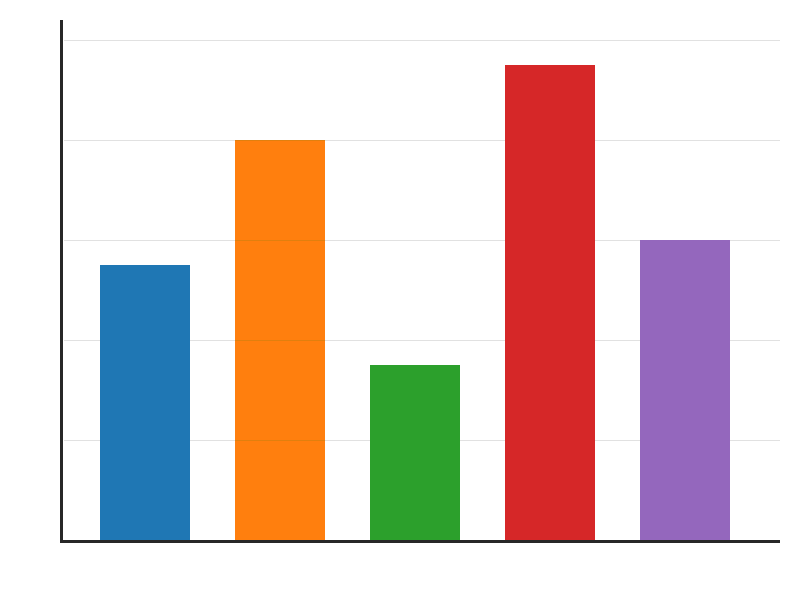
\includegraphics[width=\linewidth]{plot.png}
  \end{columns}
\end{frame}

\begin{frame}{Image with a TikZ annotation}
  \centering
  \begin{tikzpicture}
    \node[inner sep=0] (img) {
\includegraphics[width=0.6\textwidth]{photo.jpg}};
    \draw[red, very thick] (0.2, 0.1) circle (0.6);
    \node[red, font=\bfseries] at (1.6, 0.9) {Look here};
  \end{tikzpicture}

  Text under an annotated image.
\end{frame}

\begin{frame}{Full-bleed background image}
  \begin{tikzpicture}[remember picture, overlay]
    \node[opacity=0.35, inner sep=0] at (current page.center)
      {
\includegraphics[width=\paperwidth, height=\paperheight]{photo.jpg}};
  \end{tikzpicture}
  \begin{itemize}
    \item Text on top of a full-page image
    \item The image should stay in the background
  \end{itemize}
\end{frame}

\end{document}
